\documentclass{standalone}
\usepackage{tikz}
\usetikzlibrary{arrows.meta}
\tikzset{%
  >={Latex[width=2mm,length=2mm]},
  % Specifications for style of nodes:
            base/.style = {rectangle, rounded corners, draw=black,
                           minimum width=4cm, minimum height=1cm,
                           text centered, font=\sffamily},
  activityStarts/.style = {base, fill=blue!30},
       startstop/.style = {base, fill=blue!30},
    activityRuns/.style = {base, fill=green!30},
         process/.style = {base, minimum width=2.5cm, fill=orange!15,
                           font=\ttfamily},
}
\begin{document}    
% Drawing part, node distance is 1.5 cm and every node
% is prefilled with white background
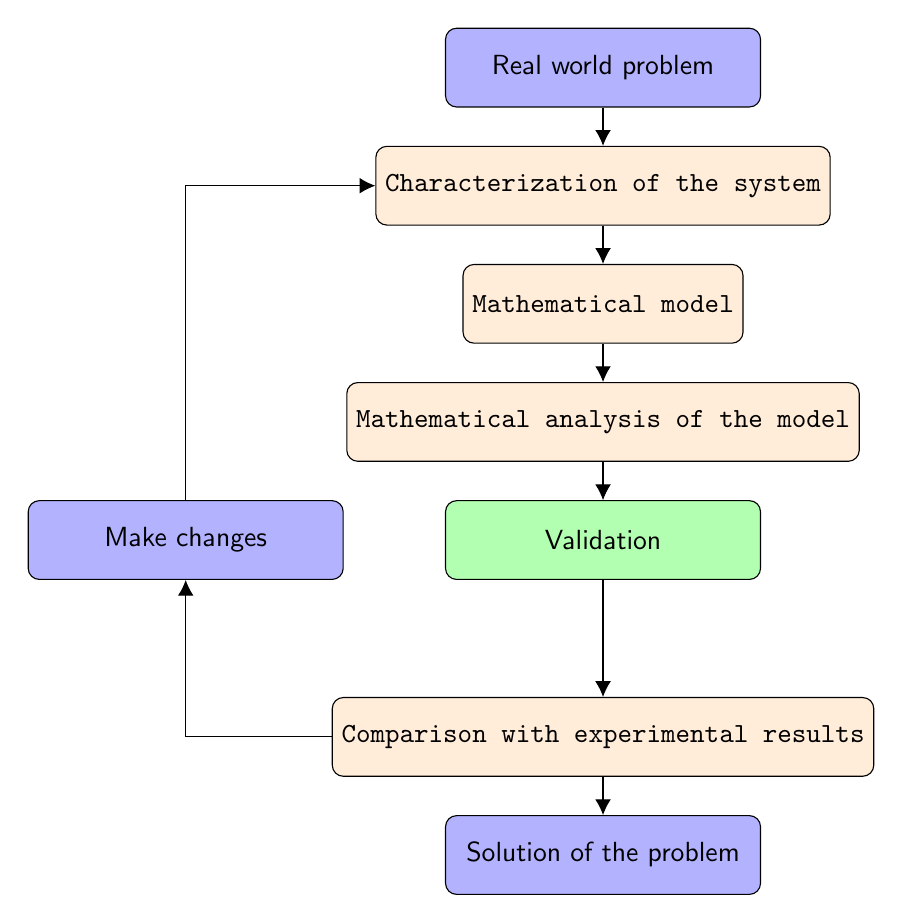
\begin{tikzpicture}[node distance=1.5cm,
    every node/.style={fill=white, font=\sffamily}, align=center]
  % Specification of nodes (position, etc.)
  \node (start)             [activityStarts]              {Real world problem};
  \node (onCreateBlock)     [process, below of=start]          {Characterization of the system};
  \node (onStartBlock)      [process, below of=onCreateBlock]   {Mathematical model};
  \node (onResumeBlock)     [process, below of=onStartBlock]   {Mathematical analysis of the model};
  \node (activityRuns)      [activityRuns, below of=onResumeBlock] {Validation};
  
  \node (onPauseBlock)      [process, below of=activityRuns, yshift=-1cm] {Comparison with experimental results};
  
   \node (ActivityDestroyed) [startstop, below of=onPauseBlock] {Solution of the problem};  
   
    \node (ActivityEnds)      [startstop, left of=activityRuns, xshift=-3.8cm] {Make changes};
    
 
  % Specification of lines between nodes specified above
  % with aditional nodes for description 
  \draw[->]             (start) -- (onCreateBlock);
  \draw[->]     (onCreateBlock) -- (onStartBlock);
  \draw[->]      (onStartBlock) -- (onResumeBlock);
  \draw[->]     (onResumeBlock) -- (activityRuns);
  \draw[->]      (activityRuns) -- (onPauseBlock);
  \draw[->]    (onPauseBlock) -- (ActivityDestroyed);
  \draw[->]      (onPauseBlock) -| (ActivityEnds);
  \draw[->]     (ActivityEnds)  |- (onCreateBlock);
  
  \end{tikzpicture}
\end{document}